
%%=============================================================================
%% H4 - Het opslagmodel van ZFS
%%=============================================================================

\chapter{Het opslagmodel van ZFS}
\label{ch:h4}

In dit hoofdstuk worden de interne bestandssysteemoperaties van ZFS wat meer toegelicht. Hierbij wordt vooral de werking van de Storage Pool Allocator en de Data Management Unit dieper uitgespit, aangezien deze componenten het beheer van data voor zich nemen.

\section{Structuur van het bestandssysteem}

Datablokken worden in ZFS voorgesteld als een boomstructuur. Vele andere bestandssystemen, zoals BTRFS op Linux, gebruiken ook boomstructuren voor het bijhouden van data \autocite{Project2017a}. De algemene werking van ZFS en andere, boomgebaseerde bestandssystemen verschillen niet zo heel veel. Echter zijn er ook eigenschappen die uniek zijn aan de manier waarop ZFS de data opslaat.

De belangrijkste elementen van een boom in de informatica zijn de volgende: de wortel (Eng.: \textit{root}), de knopen (Eng.: \textit{nodes}) en de bladeren (Eng.: \textit{leaves}) \autocite{Cohen}. Indien men bij de wortel van een ZFS-boom start, dan komt men als eerste de \textit{\"{u}berblock} tegen: dit is simpelweg een andere benaming voor de wortel van de boom. Dit datablok bevat een checksum van zichzelf en verwijst naar de andere datablokken in de boom. Afhankelijk van de sectorgrootte van een schijf, bevat een ZFS pool een zeker aantal \"{u}berblocks (een schijf waarvan de sectoren 512 bytes groot zijn geeft 128 \"{u}berblocks als resultaat) \autocite{Lucas2015}. 

Zoals reeds gezegd in Hoofdstuk \ref{ch:h3}, worden alle blokken gechecksummed om corruptie van data tegen te gaan. Deze checksums worden bewaard in het datablok zelf en in de ouder van dit blok: op deze manier is de hele ketting van datablokken gechecksummed en kan er makkelijk schade worden vastgesteld en kan deze schade eventueel worden gerepareerd. De \textit{\"{u}berblock} is het enige datablok die geen ouder heeft, en dus bewaart deze zijn checksum bij zichzelf \autocite{ZFSBonwick}.  

\section{Checksumming \& Redundantie op blokniveau}

Checksumming is een goede oplossing om corruptie te detecteren. Echter moeten er nog steeds back-upblokken aanwezig zijn om van datacorruptie te herstellen. Indien men bijvoorbeeld mirroring toepast binnen een pool, dan kan ZFS de corrupte datablokken zelf herstellen door een goede kopie van de andere schijf van de mirror te halen. Als een applicatie een aanvraag doet voor een reeks datablokken waarvan er één of meerdere beschadigd zijn, dan repareert ZFS deze datablokken automatisch; nadien worden de herstelde blokken doorgegeven aan de applicatie, zonder dat deze laatstgenoemde hier iets van merkt \autocite{ZFSBonwick}.

Maar zelfs zonder gebruik te maken van mirror VDEV's kan ZFS in sommige gevallen van corruptie herstellen. Hiervoor maakt ZFS gebruik van zogenaamde \textit{ditto blocks}: dit zijn simpelweg kopieeën van belangrijke datablokken, zoals van metadata of pool data. Deze blokken worden zo ver mogelijk uit elkaar op de schijf geplaatst, om zo de impact van datacorruptie te minimaliseren \autocite{Lucas2015}. 

\section{Transacties binnen ZFS}

ZFS is een transactioneel bestandssysteem \autocite{ZFSBonwick}. Transacties worden binnen ZFS afgehandeld door de DMU\footnote{De DMU behandelt eigenlijk enkel objecten, maar voor de eenvoud wordt er in dit hoofdstuk meestal gesproken over blokken.} en verlopen volgens een Copy-On-Write (COW) manier. Bij Copy-On-Write worden blokken nooit direct aangepast of overschreven; in plaats daarvan kopieert ZFS deze blokken eerst naar een andere locatie, om deze dan vervolgens aan te passen. Deze manier van van werken garandeert dat data op de schijf of schijven steeds consistent blijft: als er zich bijvoorbeeld een stroompanne voordoet midden in een transactie, dan kan ZFS makkelijk terugvallen op de oude boomstructuur, aangezien deze niet wordt overschreven \autocite{Lucas2015}.

\begin{figure}
        \centering
        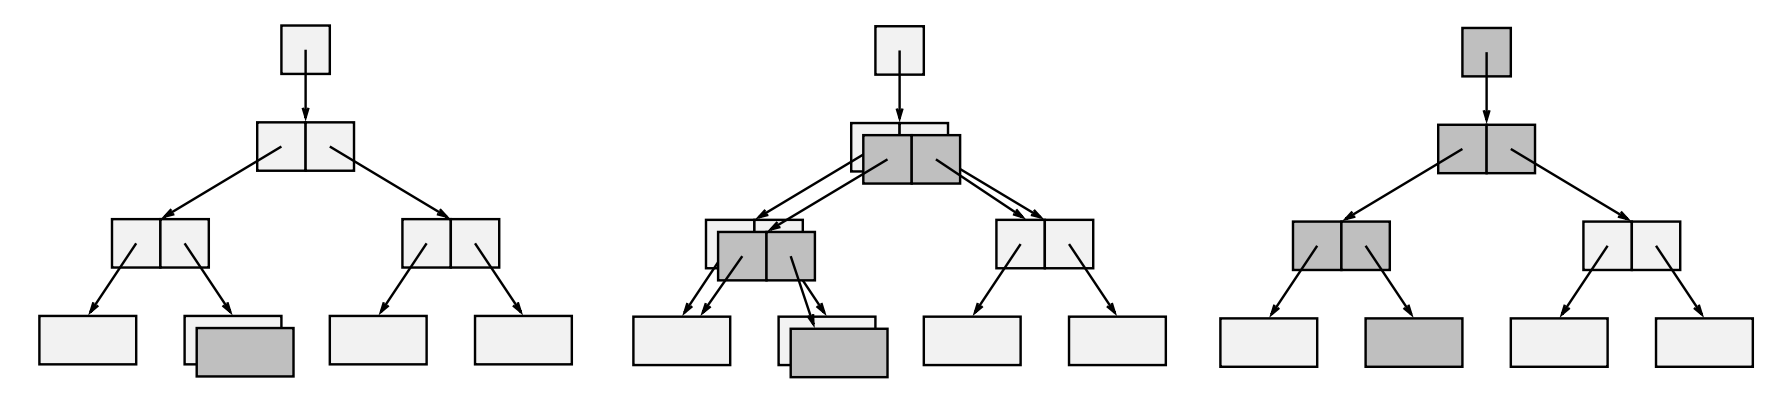
\includegraphics[width=1.0\textwidth]{h4_cow}
        \caption{Boomstructuur bij aanpassing van één datablok binnen een ZFS-transactie. Van links naar rechts: (1) Aanpassen van het datablok; (2) Aanpassen van de indirecte blokken; (3) Overschrijven van de \"{u}berblock. Alle bewerkingen gebeuren op een COW-manier. \autocite{ZFSBonwick}}
        \label{fig:bonwick_cow_illustratie}
\end{figure}

Uit de paper van \textcite{ZFSBonwick} kan men de volgende stappen opmaken die worden ondernomen bij het uitvoeren van een transactie:

\begin{enumerate}
  \item{De ZFS POSIX Layer (ZPL) krijgt de opdracht om een reeks van blokken aan te passen, te creeëren of te verwijderen. Stel dat er in dit geval één enkel datablok moet worden aangepast en dat dit blok zich in een blad van de boom bevindt. De ZPL groepeert alle wijzigingen in een transaction group (txg); hierbij moet de ZPL de wijzigingen goed groeperen opdat het bestandssysteem aan het einde van de transactie in een consistente toestand wordt achtergelaten. Voor het uitvoeren van de transactie doet de ZPL beroep op de DMU.}
  \item{De DMU start de transactie en doorzoekt de boom. De DMU heeft het blok in kwestie gevonden, kopieert het naar een nieuwe locatie en past het vervolgens aan (Copy-On-Write). Na deze aanpassing moet ook de checkum van het datablok worden herberekend.}
  \item{Aangezien andere blokken in de boom direct of indirect gekoppeld zijn aan het aangepaste datablok, moeten deze ook worden aangepast, en dit op dezelfde manier als het reeds aangepaste datablok. Ook moeten de checksums van deze blokken herberekend worden. Dit is een recursief gebeuren, en stopt bij de wortel van de boom, nl. de \"{u}berblock. }
  \item{Om de COW-eigenschappen van ZFS te garanderen, wordt het \"{u}berblock niet direct aangepast, maar wordt er geroteerd naar de volgende beschikbare \"{u}berblock. De oude en nieuwe boomstructuren worden dus a.h.w. met elkaar omgewisseld, en dit op een atomaire, transactionele manier.}
\end{enumerate}

Indien het systeem zou crashen tijdens deze transactie, dan kan de \"{u}berblock corrupt raken. Aangezien corruptie kan worden gedetecteerd met behulp van checksums, kan er eenvoudig worden teruggevallen op een oudere versie van een \"{u}berblock \autocite{ZFSBonwick}.


